\title{Assignment 1: CS 215 \\ Solutions}
\author{
	Neeraj Dhake \\ 150050022
	\and
	Rohit Kumar Jena \\ 150050061
}
\date{10th August 2016}

\documentclass[11pt]{article}

\usepackage{amsmath}
\usepackage{amssymb}
\usepackage{float}
\usepackage{hyperref}
\usepackage{ulem}
\usepackage[margin=0.5in]{geometry}
% include graphics for images
\usepackage{graphicx}
\graphicspath{{../}}
% begin document
\begin{document}
\pagenumbering{gobble}
\maketitle
\newpage
\pagenumbering{arabic}

\textbf{Honor Code:} 
\begin{itemize}
\item We pledge by our honor that we will complete the assignments in a legitimate way and will not provide or recieve any unauthorized help. 
\end{itemize}
\vspace{5mm}
\textbf{Instructions to run code: }
\begin{itemize}
	\item {
		For Question 4, the corresponding files are \textit{hw1\_q4.m} (to run the file and generate plots as well as give the relative errors for both the median and the mean) and \textit{neighbours.m} (to generate the neighbours of the array at a given index .i.e. if index is 14 then it will return \textbf{z(6:22)} ). \\
		To run the program, simply type \textit{hw1\_q4} from the MATLAB command line.
	} 
	\item {
		For Question 5, the corresponding files are \textit{hw1\_q5.m} (to read the original array from the file named \textit{input\_array.txt} and compute the mean, median, and the standard deviation). Then it prompts the user to enter the new data value. It uses the \textit{UpdateMean.m}, \textit{UpdateMedian.m}, and \textit{UpdateStd.m} files to compute the new mean, new median and new standard deviation from the old values. \\
		To run the file, simply type \textit{hw1\_q5} from the MATLAB command line. Make sure you have a file named \textit{input\_array.txt} containing the array elements in \textbf{one line (row vector)} .
		Or you can just use the UpdateMean, UpdateMedian and UpdateStd files as you wish. Make sure the array A is a row vector.
	}
	\item {
		\textbf{Note:} The code works perfectly both in MATLAB R2015\_B version as well as in Octave. A file \textit{input\_arrray.txt} is present with a 100-element array for Question 5. You can obviously change the data, but please keep the array as a row vector.
	} 
\end{itemize}
% \\
% \\
\textbf{Solutions: }
% solutions begin here
\begin{enumerate}
	\item{
	Let $\mu$ = mean and $v$ = median of the dataset $\{x_i\}_{i=1}^{N}$ containing $N$ data points.
	$$ \left|\mu - v\right| = \left|\frac{\sum_{i=1}^{N}(x_i - v)}{N}\right| \leq \frac{\sum_{i=1}^{N}\left|x_i - v\right|}{N}$$
	By Triangular Inequality,
	$$ \left|\frac{\sum_{i=1}^{N}(x_i - v)}{N}\right| \leq \frac{\sum_{i=1}^{N}\left|x_i - v\right|}{N} $$ 
	$$ \implies  \frac{\sum_{i=1}^{N}\left|x_i - v\right|}{N} \leq \frac{\sum_{i=1}^{N}\left|x_i - \mu \right|}{N} $$
	\hfill(the value for which $ \frac{\sum_{i=1}^{N}\left|x_i - x\right|}{N} $  is minimum is when $x$ = median) \\
	Now, \\
	$$ {\Bigg(\frac{\sum_{i=1}^{N}\left|x_i -\mu\right|}{N}\Bigg)}^2 \leq \frac{\sum_{i=1}^{N}{\left|x_i -\mu\right|}^2}{N} \leq \frac{\sum_{i=1}^{N}{\left|x_i -\mu\right|}^2}{N-1} = \sigma^2 $$
	\hfill{ (by RMS-AM inequality ($\frac{(\sum_{i=1}^N{a_i})}{N} \leq \sqrt{\frac{\sum_{i=1}^N{a_i^2}}{N}}, \forall a_i > 0$))} \\
	$$ \therefore \left|\mu - v\right| \leq \sigma $$
	} 


	\item {
	Given 4 datasets $\{x_i\}_{i=1}^{N}$, $\{y_i\}_{i=1}^{N}$ , $\{z_i\}_{i=1}^{N}$, and $\{w_i\}_{i=1}^{N}$ such that,
	$$ z_i = ax_i+b $$ $$ w_i = cy_i+d $$ 
	Using the definition of correlation coefficient, we have,
	$$ r(x,y) = \frac{\sum_{i=1}^{N}{(x_i-\mu_x)(y_i-\mu_y)}}{(N-1)\sigma_x\sigma_y} $$
	$$ r(z,w) = \frac{\sum_{i=1}^{N}{(z_i-\mu_z)(w_i-\mu_w)}}{(N-1)\sigma_z \cdot \sigma_w} $$
	\text{Now if mean of } $\{x_i\}_{i=1}^{N} = \mu_x $\text{ then mean of } $\{z_i\}_{i=1}^{N} = a\mu_x + b$ \text{ , and similarly mean of } $\{w_i\}_{i=1}^{N} = a\mu_y + b$.\\

	Substituting the values of $z_i,\mu_z,w_i,\mu_w$ in the second equation, we get, 
	$$
	r(z,w) = \frac{\sum_{i=1}^{N}{[(ax_i+b)-(a\mu_x+b)] \cdot [(cy_i+d)-(c\mu_y+d)]}}{(N-1)\left|a\right|\sigma_x \cdot \left|c\right|\sigma_y} 
	$$
	$$ =  \frac{\sum_{i=1}^{N}{a(x_i-\mu_x) \cdot c(y_i-\mu_y)}}{(N-1)\left|a\right|\sigma_x \cdot \left|c\right|\sigma_y}$$
	$$ =  sgn(ac)\cdot\frac{\sum_{i=1}^{N}{(x_i-\mu_x)(y_i-\mu_y)}}{(N-1)\sigma_x\sigma_y} $$
	Where $sgn(ac)$ denotes the signum function. \\
	Now, substituting the definition of $r(x,y)$, we have, \\
	$$ r(z,w) = sgn(ac) \cdot r(x,y) $$
	When the sign of $ac$ is positive, i.e. when both $a$ and $c$ are positive or negative, we have $sgn(ac) = 1$, and hence $r(z,w) = r(x,y)$. \\
	When the sign of $ac$ is negative, i.e. when the sign of $a$ and $c$ are opposite, we have $sgn(ac) = -1$, and hence $r(z,w) = -r(x,y)$. \\
	}

	\item {
	Let $x_i$ be the datapoints of a dataset $\{x_i\}_{i=1}^{N}$ with mean $\mu$. \\
	So, we have the following inequality,
	$$	\left|x_i - \mu\right| \leq \sqrt{\sum_{i=1}^{N}{\left|x_i -\mu\right|}^2} $$
		\text{This can easily be shown as follows: }
	$$	\left|x_i -\mu\right|^2 \leq \sum_{i=1}^{N}{\left|x_i -\mu\right|}^2 $$ \\
		\text{Since both R.H.S and L.H.S are positive, taking square root on both sides gives the required result.}
	$$	\left|x_i - \mu\right| \leq \sigma\sqrt{n-1} $$ 
		\hfill \text{ Q.E.D.}
	}

	\item {
		The corresponding file is \textit{hw1\_q4.m}. The values obtained are as follows - \\
		For error in [5,10] , \\
		\textbf{Relative median error} - 9.29 x $10^{-2}$\% \\
		\textbf{Relative mean error} - 1.53\% \\ \\
		For error in [100,120], \\
		\textbf{Relative median error} - 9.84 x $10^{-2}$\% \\
		\textbf{Relative mean error} - 361.75\% \\

		\textbf{Explanation: } \\
		As we can see, the errors in mean increase as the corrupt values increase in magnitude. The moving median filtering produced a better relative mean squared error. This is because median is way less sensitive to outliers than the mean. 
		Also since the ratio of number of corrupted points to the number of total points is very less , even sharp peaks in those points can drastically change the mean of the neighbouring points. But the median of neighbouring points is not affected unless the corrupted values turn out to be the median of the set neighbouring it. 
		Here is the plots corresponding to the errors belonging to [5,10] and [100,120].
		
		\textbf{Note: }The same plots can be easily generated by running the \textit{hw1\_q4.m} file from MATLAB command line.
		\begin{figure}[H]
		\caption{Plot with error $\in$ [5,10]}
		\centering
		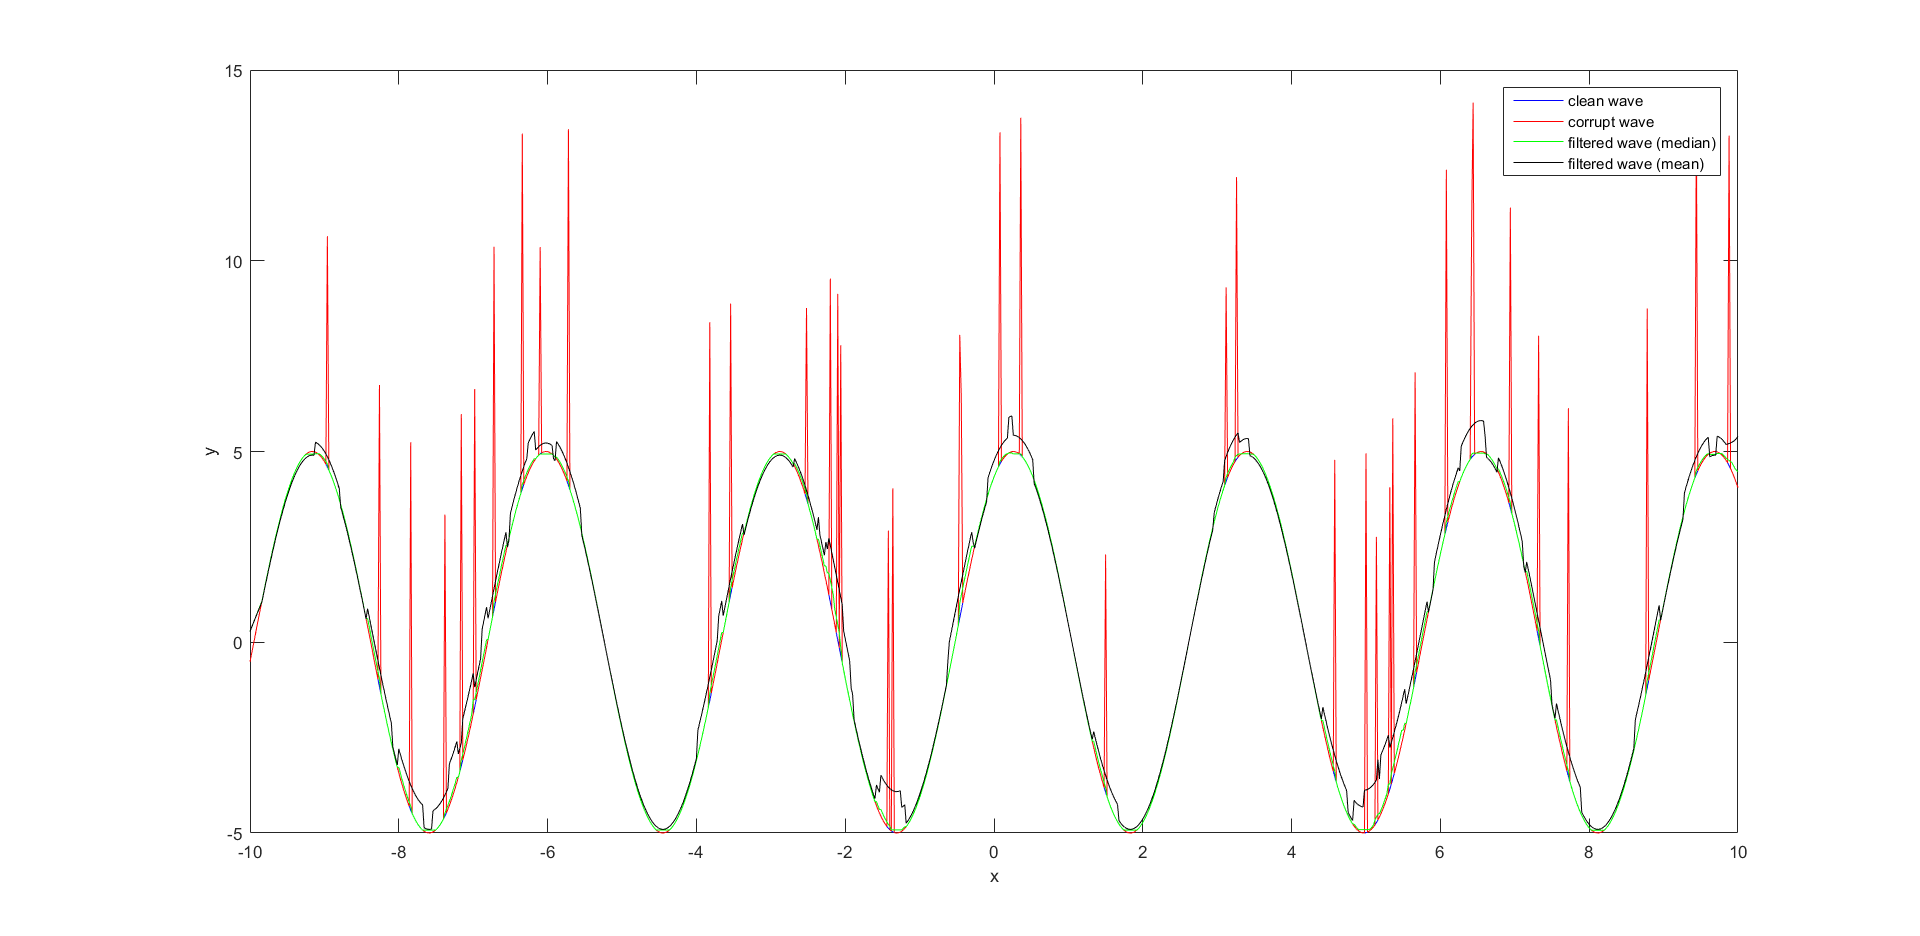
\includegraphics[width=\textwidth]{error_1}
		\end{figure}
		\begin{figure}[H]
		\caption{Plot with error $\in$ [100,120]}
		\centering
		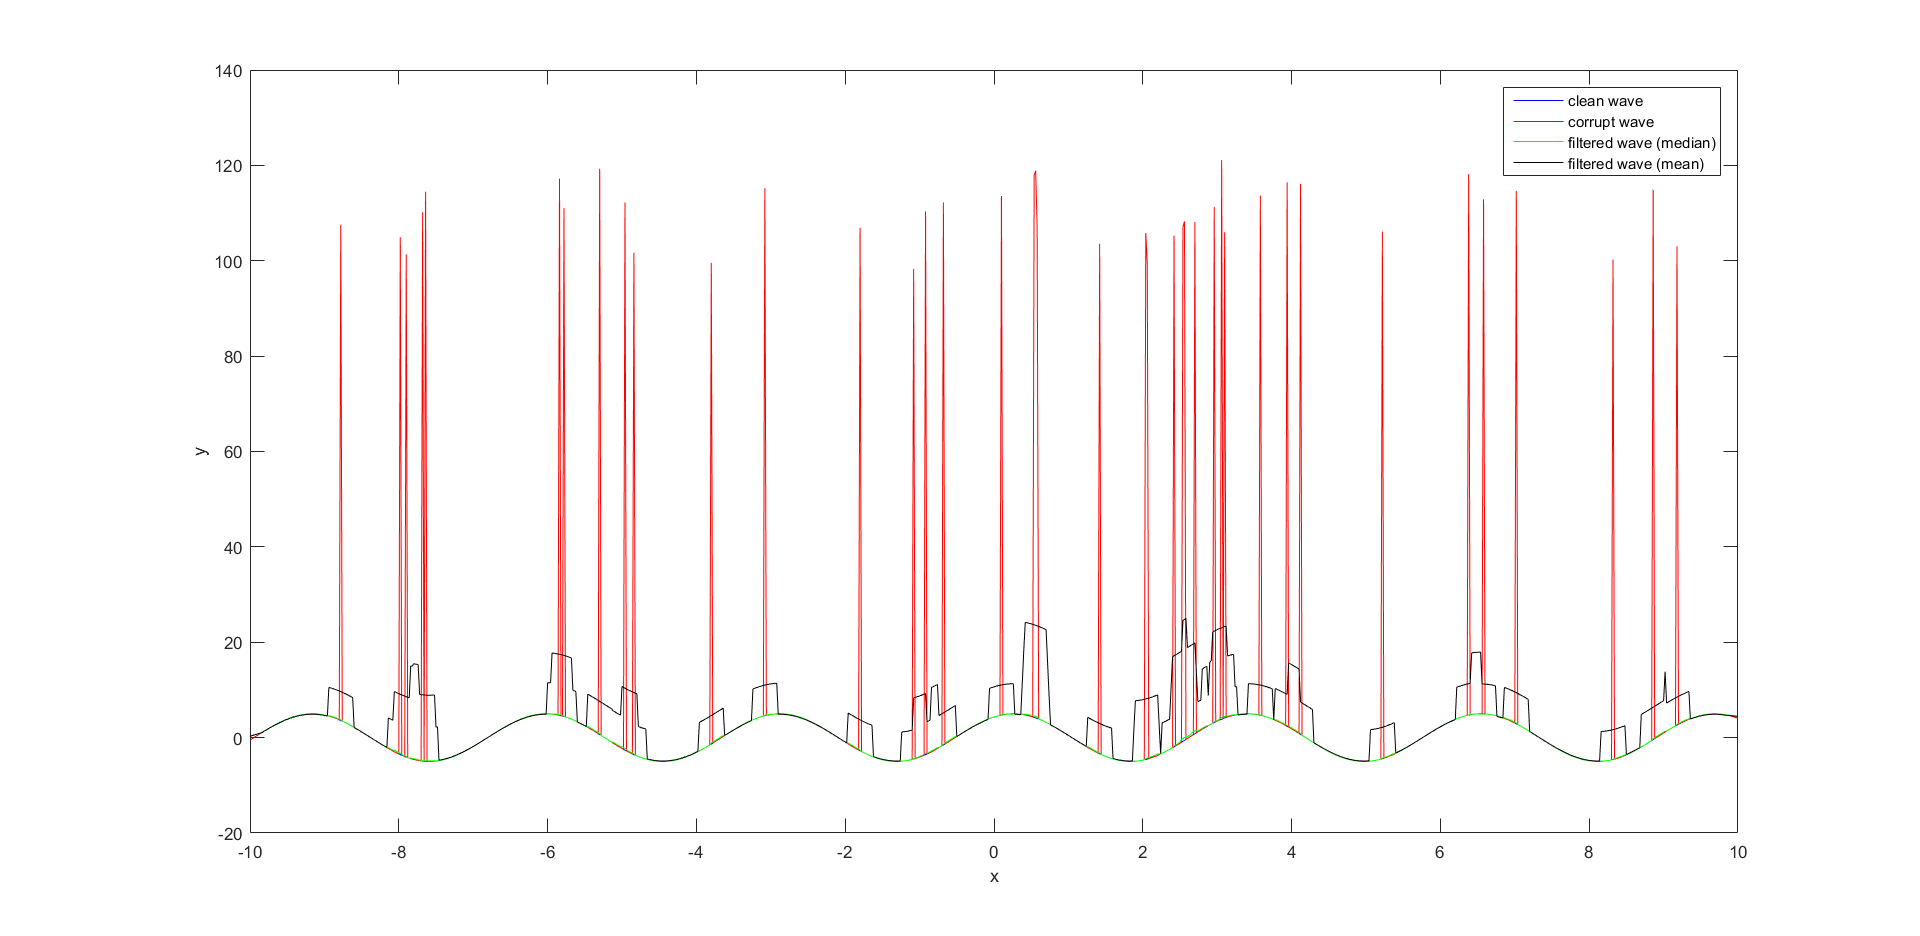
\includegraphics[width=\textwidth]{error_2}
		\end{figure}
 	}

	\item {
	Let $ \bar{a} $ denote the mean of a dataset $\{a_i\}_{i=1}^{N}$ having $N$ datapoints. \\ 
	Now, we have, \\
	$$ \bar{a} = \frac{\sum_{i=1}^N{a_i}}{N} $$ \\
	After we add a new element, say $z$, the new mean becomes, \\
	$$\bar{a}_{new} = \frac{\sum_{i=1}^{N+1}{a_i}}{N+1} = \frac{(\sum_{i=1}^{N}{a_i} )+ z}{N+1} = \frac{N\bar{a}+z}{N+1} $$
	$\therefore$ We have the value of $\bar{a}_{new}$ in terms of $\bar{a},N,z$. \\ \\

	For the given data, let the standard deviation be denoted by $\sigma$. So we have, \\
	$$\sigma^2 = \frac{\sum_{i=1}^{N}{(x_i-\bar{x})^2}}{N-1} = \frac{(\sum_{i=1}^{N}{x_i^2}) - N\bar{x}^2}{N-1}$$
	
	After adding a new value $z$ to the data, we have a new value $\sigma_{new}$ denoted by, \\
	$$ \sigma_{new}^2 = \frac{\sum_{i=1}^{N+1}{(x_i-\bar{x})^2}}{N} = \frac{(\sum_{i=1}^{N+1}{x_i^2}) - (N+1)\bar{x}_{new}^2}{N} $$
	
	Using the value of $\sigma^2$, we apply the following substitution, \\
	$$ \sum_{i=1}^{N}{x_i^2} = (N-1)\sigma^2 + N\bar{x}^2 $$

	We get the following equation, \\
	$$ \sigma_{new}^2  = \frac{(N-1)\sigma^2 + N\bar{x}^2 + z^2 - (N+1)\bar{x}_{new}^2}{N} $$

	$\therefore$ We have the value of $\sigma_{new}$ in terms of $\sigma$, $\bar{x}$, $\bar{x}_{new}, z$, and $N$. \\
	}
\end{enumerate}

\end{document}